\documentclass{article}
\usepackage{times}
\usepackage{graphicx}
\usepackage{subfigure}
\usepackage{natbib}
\usepackage{algorithm}
\usepackage{algorithmic}
\usepackage{hyperref}
\newcommand{\theHalgorithm}{\arabic{algorithm}}
\usepackage[accepted]{icml2014}
\icmltitlerunning{Predicting Cervix Types with Convolutional Neural Networks}


\begin{document}
\twocolumn[
\icmltitle{Predicting Cervix Types with Convolutional Neural Networks}
\icmlauthor{Lan-Anh Ngo-Quy}{lngoquy1@swarthmore.edu}
\icmlauthor{Dina Ginzburg}{dginzbu1@swarthmore.edu}
\icmladdress{Swarthmore College, \\ 500 College Ave, \\Swarthmore, PA, 19081}
\vskip 0.3in
]


\begin{abstract}
Cervical cancer is easily treatable when detected in its pre-cancerous
stage. Many women, particularly those who are low-income, benefit from
programs which identify and treat cervical cancer within a single
visit. Depending on their cervix type, further treatment may be
required for the patient. This decision is very important, and since
identifying the transformation zones is not an easy task for
healthcare providers, developing an algorithm to correctly identify
cervix type based on cervical images is critical, especially for
related research dealing with large datasets.  In this paper we will
present our solution to predicting the cervix types. First, we
segmented ROI to exclude irrelevant information while preserving the
cervix in its entirety.   The
processed images were then split into training, tuning and test sets
and fed into a Convolutional Neural Network (CNN). We
also implemented the Bag of Words method and a Multi-Layer Perceptron,
to compare our CNN's performance to other classifiers. We found that
Bag of Words performed the best with accuracy rate of 56.78\%, while CNN reaches an accuracy rate of
54.4\%, which although significantly better than chance and better
than average performance of the 3 methods (51.85\%), is not accurate
enough for our classifier to be reliable. Further work to boost the
classifier's performance would be better data augmentation, image
segmentation methods that match the cervix boundary more closely and
implementing fine-tuning with weights from a pre-trained CNN.
\end{abstract}

\section{Introduction}
\label{introduction}

\begin{figure}[ht]
  \vskip 0.2in
  \begin{center}
  \centerline{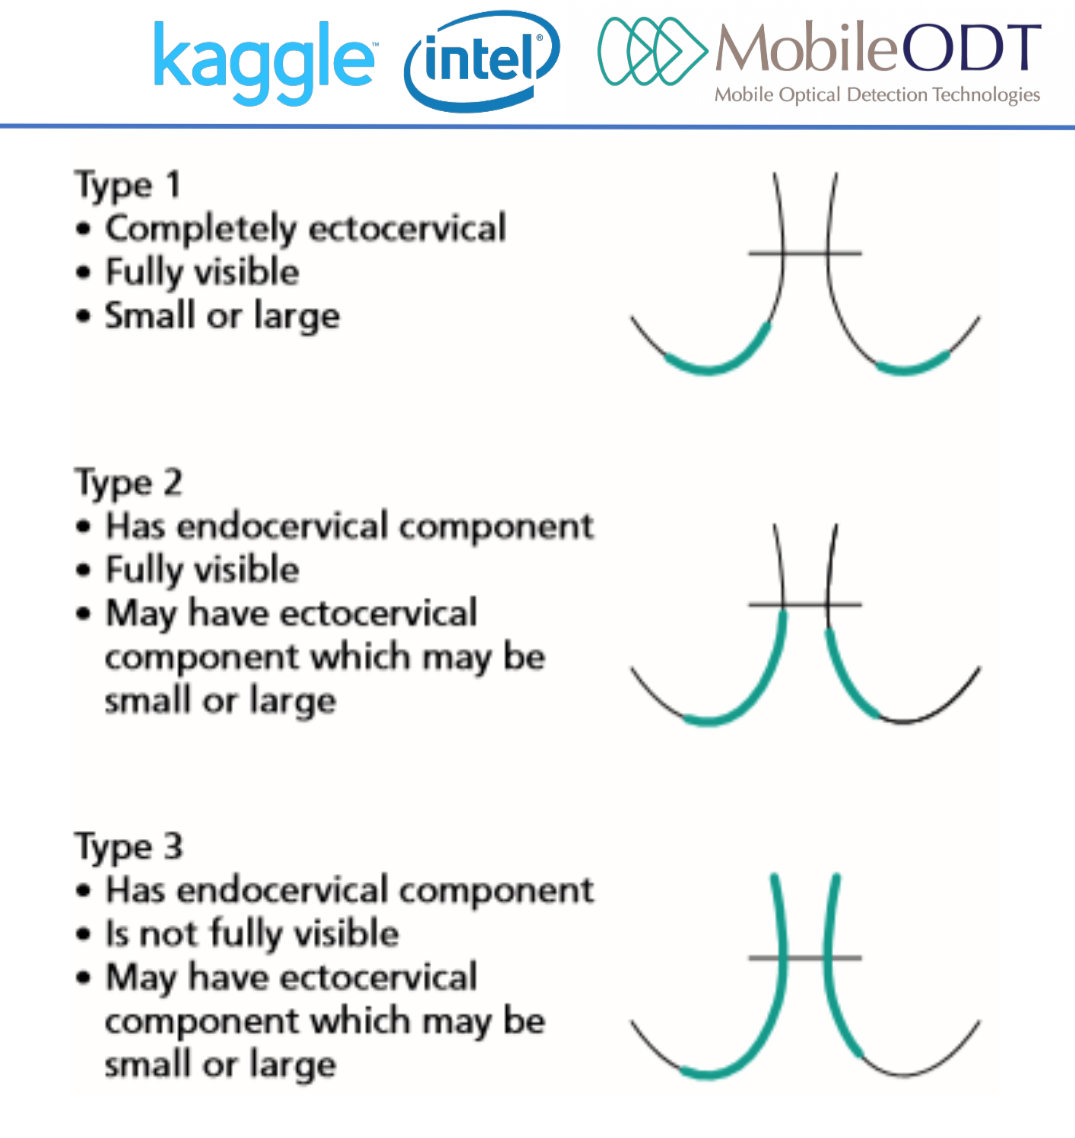
\includegraphics[width=\columnwidth]{cervixtype}}
  \caption {Three types of cervix.}
  \label{three}
  \end{center}
  \vskip -0.2in
\end{figure}

Treatment for cervical cancer is relatively simple when it is detected
in a pre-cancerous stage. However, many health care specialists lack
the expertise to determine the appropriate method of treatment-- which
can vary wildly based on each patient’s unique physiology. Applying
the wrong treatment can not only increase health risks for the
patient, but is also very costly. MobileODT, a company which seeks to
prevent cervical cancer by developing and selling the Enhanced Visual
Assessment (EVA) System. The EVA system is a digital toolkit for
health care workers, which includes a mobile-phone based medical
device designed to use biomedical optics to screen and treat patients
for cervical cancer \cite{kaggle}. MobileODT and Intel have decided to
partner in a Kaggle competition with the purpose of developing an
algorithm which accurately predicts a patient’s cervix type based on
cervix images. We tried three different approaches to solving this
problem: a CNN, Bag of Words, and a Multi-Layer Perceptron. We found that we were able to get Bag of Words to perform the best, although all three methods had lackluster results.

\begin{figure}[ht]
  \vskip 0.2in
  \begin{center}
  \centerline{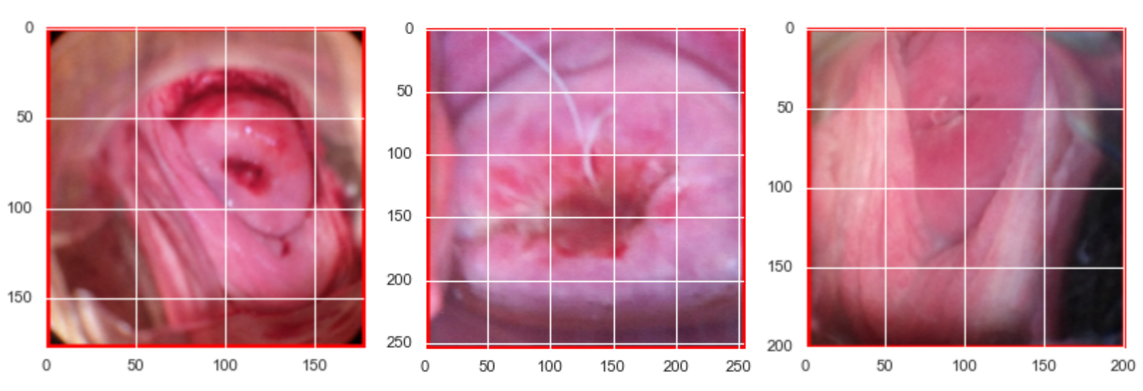
\includegraphics[width=\columnwidth]{types123}}
  \caption {Cervigrams from left to right: type 1, type 2, type 3.}
  \label{cervigram}
  \end{center}
  \vskip -0.2in
\end{figure}

Most Cervical cancers begin in the cells of the transformation zone
(an area of the cervix). There are three cervix types and each one has
a different transformation zone location. It is important to know what
the cervix type is because cervix types 2 and 3 might include hidden
lesions and require different treatment. However the transformation
zones aren't always visible and they're difficult to identify for
health care providers, so an algorithm-based approach can greatly aid
real-time determinations about patient treatment
\cite{kaggle}. Fig. (2) shows an example for each type of cervix in
the dataset. 

We decided to try a combination of image preprocessing and a Convolutional Neural Network (CNN) to classify the cervix images. We used segmentation on the data to get the Region of Interest for each image, and eliminated white noise. We used a combination of methods outlined by Greenspan and a kaggle kernel authored by the user "chattob". We then fed the data into a CNN, experimenting with different types of layers and hyperparameters. We drew on Srivastava's work on Dropout layers and Ioffe's work on Batch Normalization to reduce overfitting in our CNN. We also implemented Bag of Words and a Multi-Layer Perceptron, and compared accuracy rates among these three methods.

We were surprised to find that despite tinkering with hyperparameters and running multiple tests with different architectures, our Convolutional Neural Network only performed better than the Multi-Layer Perceptron. In fact, Bag of Words had the highest accuracy of all three methods we implemented. However, none of the three methods were able to get exceptionally high accuracy on the test set, with Bag of Words reaching only 56.78\% accuracy.


\section{Methods}
Our algorithm for cervix prediction consists of image preprocessing to find the Region of Interest in each image and reduce noise in the image. The processed data is then fed into a Convolutional Neural Network. To compare the performance of our implementation of the CNN, we also implemented the Bag of Visual Words (BoW) method and a Multi-layer Perceptron (MLP).

\subsection{Image Preprocessing}

Before the images can be fed into any classifying algorithm, they need
to go through a preprocessing step which will produce smaller
sub-images containing only the cervix area, our Region of Interest
(ROI). Challenges in identifying the correct region include lack of
distinct boundaries among different tissues, the small color range,
reflection artifacts, large variability in the viewing angles, cervix
sizes and tissue types presented in the images. A summary of the image
segmentation process is illustrated by Fig. (3). To exclude the black circular frames often seen in the cervigrams, our method cropped the circle out by finding the maximum continuous rectangle area. Since the cervix region has a relatively pink color and should be at the center of the cervigram, in function Ra\_space we chose to represent each pixel of the image by 2 values: the minimum of the a color of the Lab color space a = 150 and the pixel’s red channel value, and the pixel’s distance R from the image center. Each image is then separated into 2 clusters using Gaussian Mixture Model in 2-dimensional space. The ROI will then be the largest connected component among the pixels belonging to the cluster with the highest a and the lowest R values \cite{kernel}. 

\begin{figure}[ht]
  \vskip 0.2in
  \begin{center}
  \centerline{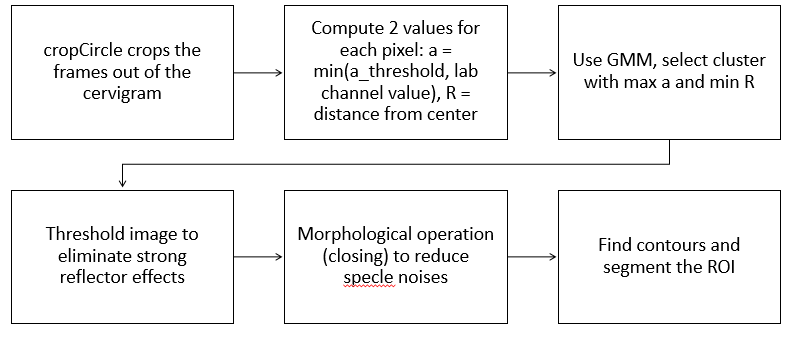
\includegraphics[width=\columnwidth]{flowchart}}
  \caption {Segmentation algorithm.}
  \label{cnn}
  \end{center}
  \vskip -0.2in
\end{figure}

To make the image less noisy, pixels in small and bright discontinuous regions (SR) caused by strong reflectors on the cervix surface are detected by thresholding. We created a thresholded mask and removed those areas which were above the threshol by setting them equal to (0, 0, 0). This prevents these areas from interfering with the content analysis of the surrounding regions. Additionally, Morphological operation closing was used to remove speckle noises. Our final preprocessing step was to find contours which we then use to choose our width and height for our ROI \cite{autodetect}.

\begin{figure}[ht]
  \vskip 0.2in
  \begin{center}
  \centerline{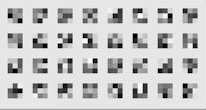
\includegraphics[width=\columnwidth]{firstconvlayer}}
  \caption {Kernels for the first Convolutional Layer of our CNN architectures.}
  \label{kernels}
  \end{center}
  \vskip -0.2in
\end{figure}

\subsection{Convolutional Neural Networks}
Convolutional Neural Networks are very similar to regular Neural Networks: they are made up of neurons with weights and biases, which take a set of inputs and perform a dot product. However, CNNs make the explicit assumption that the inputs are images. This allows for a more efficient forward function and reduces the number of parameters in the network. In a regular Neural Network, each neuron is fully connected to each neuron in the previous layer. This does not scale well to images, where each fully connected neuron would require width*height*3 weights. CNNs solve this problem by constraining the architecture - each layer of the network arranges its neurons three-dimensionally by width, height, and depth. Neurons in each layer are only connected to a small patch of the previous layer. For our project, we used the Keras neural network library \cite{cs231n}.

Our CNN used three built-in Keras layers: a Convolution layer (Conv),
a Pooling layer (Pooling), and a Fully-Connected layer (FC). The
Convolution layer is the main component of a CNN, doing most of the
heavy computational work. Each parameter in this layer is a learnable
filter (with height and width much smaller than the input image) which
is convolved along the width and height of the image during the
forward pass. This process produces a 2-dimensional activation map
which gives the filter response at each position in the image. The
network will learn filters that activate when they see certain
features in the image. Fig. (4) shows the kernels for the first
convolutional layer of our best-performing CNN model. The Pooling
layer is inserted after a Convolution layer in order to reduce the
size of the representation. This results in not only a reduced number
of parameters and computation time, but also helps to prevent
overfitting. The final Fully-Connected layer functions just like a
regular fully-connected Neural Network. These layers can be arranged
in any order, sometimes with many layers of Convolution and
Pooling. \cite{cs231n}. Fig. (5) demonstrates an example arrangement
of the layers in a CNN. 




\begin{figure*}[ht]
\vskip 0.2in
\begin{center}
\centerline{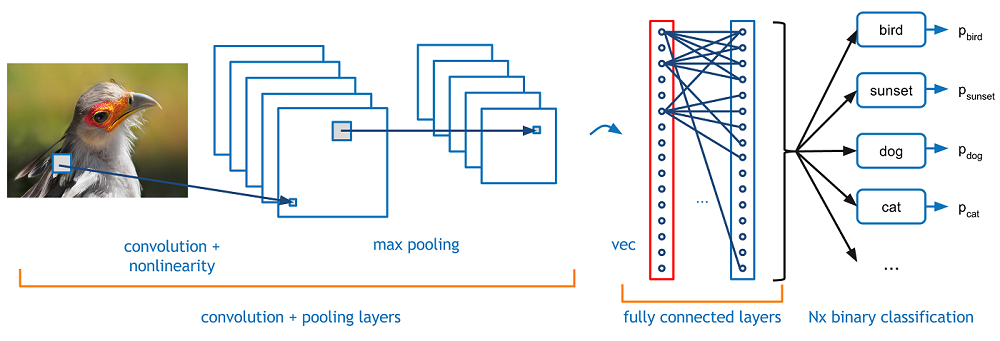
\includegraphics[scale = .8]{cnn}}
\caption{A Convolutional Neural Network with Convolution, Pooling, and Fully Connected layers.}
\label{cnn1}
\end{center}
\vskip -0.2in
\end{figure*}

\begin{figure}[ht]
  \vskip 0.2in
  \begin{center}
  \centerline{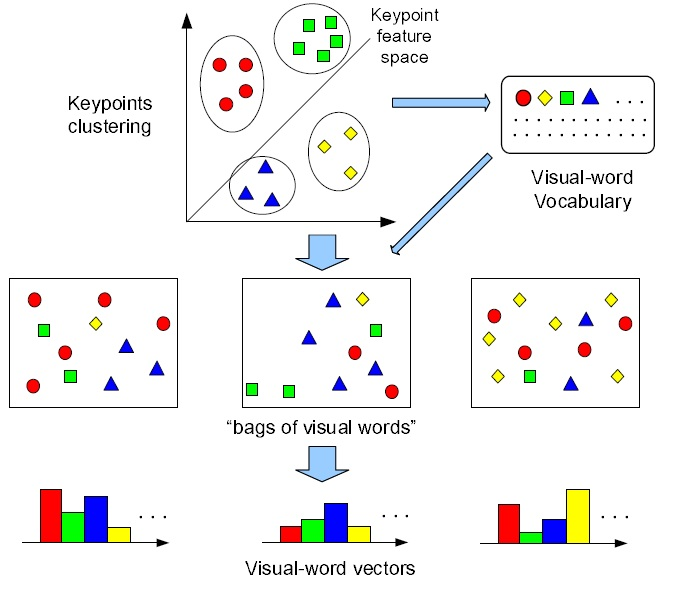
\includegraphics[width=\columnwidth]{bagofwords}}
  \caption {Bag of Words algorithm.}
  \label{bag}
  \end{center}
  \vskip -0.2in
\end{figure}

Additional layers used our architecture were BatchNormalization and Dropout layers. In deep neural networks, the changes in parameters of the previous layers will result in a different distribution of each layer’s input. This requires lower learning rates and careful initialization, slowing down the training \cite{ioffe}. A method to address this problem is normalizing layer inputs, thus following common practice \cite{cs231n}, we inserted a Batch Normalization layer immediately after our convolutional layer. The Dropout layer prevents overfitting during training by randomly dropping units along with their connections from the neural network \cite{drop}. In the tests conducted, we added a Dropout layer after the convolutional layer and the BatchNormalization layer. 





\subsubsection{Parameters for CNNs}
Convolutional Neural Networks require that we provide certain parameters. For the Convolutional layer, $W$ is the input volume - or the size (width*height*depth) of the image. $F$ is the receptive field size - or the size of the filter in the Convolution layer. $S$ is stride - or how many pixels we move the filter each time we slide it across the image. Sometimes it is convenient to pad the input volume with zeros around the border - the size of this border is $P$. These variables will be referenced later in this paper \cite{cs231n}.



\subsection{Bag of Words}
To compare our CNN performance to other methods, we also implemented
Bag of Words (BOWs) for images, fig. (6) illustrates the steps taken
in this algorithm. BOWs works by treating each image as a document and each image feature as a word. Once features are detected (by sliding a kernel along the images), they are represented by vectors called feature descriptors. BOWs functions by creating a codebook which converts these vectors into “codewords”, which can be representative of multiple vectors. To create the codebook, we used K-means clustering on the vectors, and chose the centers of each cluster as the codeword. An image is then represented by the histogram of the codewords, which allows us to classify the image based on its histogram using a multi-class AdaBoost classifier from sk-learn \cite{bag}.


\subsection{Multi-Layer Perceptron}
The other method we implemented to compare our CNN performance to was the Multi-Layer Perceptron (MLP). An MLP is an artificial neural network with multiple layers of nodes. Each layer is fully connected to the next one. Our implementation used a single hidden layer with 16 hidden nodes. 

\section{Experiments}

We used the datasets downloaded from kaggle’s Intel \& MobileODT Cervical Cancer Screening \href{https://www.kaggle.com/c/intel-mobileodt-cervical-cancer-screening}{https://www.kaggle.com/c/intel-mobileodt-cervical-cancer-screening}. The datasets consist of 250 images labeled Type 1, 781 images labeled Type 2, and 450 images labeled Type 3. Most of the images contain irrelevant details to our training algorithm such as medical devices and unidentifiable tissue, so we used the method specified by Greenspan et. al. \cite{autodetect} to segment the cervix as smaller sub-images containing only the region of interest (ROI). The images after segmentation had different dimensions, so we chose the minimum dimension (58x58) to resize all of them. The final preprocessing step was converting the data type to float32 and normalizing the data to the range of [0, 1].  

Even though the segmentation method correctly identified the ROI for most of the images, there are some images that still have parts of medical devices. The sizes vary a lot among the images (the largest size after segmentation is 256, but all images are then scaled to 58x58 - the minimum shape detected).  Fig. (7) shows an example of two images: the one on the left is properly segmented, while the one on the right is an example of poor segmentation.

Since only the labels for the training set are provided, for
supervised learning we used cross validation. We first split the
images into train and test sets by a ratio of 2:1. To choose the best
set of hyperparameters we further split X\_train into a training set
and tuning set by a ratio of 4:1. Thus, the final training, tuning,
and test sets consist of 793, 199 and 489 images. For feeding X\_train and Y\_train into the CNN, we needed to convert
our 1-dimensional label arrays Y\_train and Y\_test into 3-dimensional
label matrices. 

\begin{figure}[ht]
  \vskip 0.2in
  \begin{center}
  \centerline{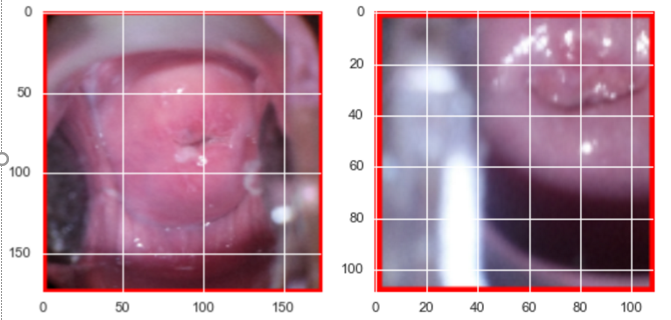
\includegraphics[width=\columnwidth]{cervix}}
  \caption {Two examples of image segmentation. Left example worked correctly, while right example failed.}
  \label{badimages}
  \end{center}
  \vskip -0.2in
\end{figure}

To understand our CNN net better, we conducted several timed tests to
figure out what should be the best set of hyperparameters. For the
images of size 58 x 58, we chose to set the receptive field size F =
3, with stride S = 0 and padding on the border of the images B =
1. The choice of a small receptive field size and 0 stride is to avoid
losing too much information. The size of the kernel for MaxPooling
layer was set to (2,2) since any larger number would demand K to be
larger in the previous convolutional layer(s), which would make the
model prone to overfitting to the training data. All of the layers we
used in the testing architectures used 'relu' activation except for
the last FC layer when softmax was used instead. We adjusted the
number(s) of kernels K for the convolutional layer, the number of
output nodes for the FC layer, changed the batch size, and rearranged
the architecture of the neural networks. For the FC before the last
one, we used weight regularization to further prevent overfitting. We run all the testing
architectures with batch size of 10 in 8 epochs, unless specified
otherwise. Our model's architectures for testing is summarized by
Table. (1). 


\begin{table}[h!]
  \caption{Summary of the CNN architectures used for testing}
  \label{tab:format}
  \vskip 0.15in
  \begin{center}
 \begin{small}
 \begin{sc}
 \begin{tabular}{lcccccr}
 \hline
 \abovespace\belowspace
Architecture & Layers\\
\hline
\abovespace
CNN0 & Conv Layer(K) $\rightarrow$ Pooling\\
 &  $\rightarrow$ BatchNormalization $\rightarrow$ Flatten \\
 & $\rightarrow$ FC(D) $\rightarrow$ BatchNormalization \\
 \belowspace
 & $\rightarrow$ FC(softmax, 3)\\
\hline
\abovespace
CNN1 & Conv Layer(K) $\rightarrow$ Pooling \\
 & $\rightarrow$ BatchNormalization $\rightarrow$ \\
 & Dropout(0.25) $\rightarrow$ Flatten $\rightarrow$ \\
 & FC(D) $\rightarrow$ BatchNormalization\\
\belowspace
 & $\rightarrow$ Dropout(0.25) $\rightarrow$ FC(softmax, 3)\\
\hline
\abovespace
CNN2 & Conv Layer(K) $\rightarrow$ Pooling \\
 & $\rightarrow$ BatchNormalization $\rightarrow$ \\
 & Dropout(0.25) $\rightarrow$ Conv Layer(16) $\rightarrow$ \\
 & Pooling$\rightarrow$ BatchNormalization$\rightarrow$ \\
 & Flatten $\rightarrow$ FC(D) $\rightarrow$ \\
 & BatchNormalization $\rightarrow$ Dropout(0.25)\\
\belowspace
 &  $\rightarrow$ FC(softmax, 3)\\
\hline
\abovespace
CNN3 & Conv Layer(K) $\rightarrow$ Pooling \\
 & $\rightarrow$ BatchNormalization $\rightarrow$ \\
 & Dropout(0.25) $\rightarrow$ Conv Layer(16) \\
 & Pooling $\rightarrow$ BatchNormalization \\
 & $\rightarrow$ Conv Layer(8) $\rightarrow$ \\
 & Pooling$\rightarrow$ BatchNormalization $\rightarrow$ \\
 & Flatten $\rightarrow$ FC(D)$\rightarrow$ \\
 & BatchNormalization $\rightarrow$ Dropout(0.25)\\
\belowspace
 & $\rightarrow$ FC(softmax, 3)\\
\hline
\abovespace
CNN4 & Same as CNN1 but without \\
\belowspace
 & BatchNormalization layer\\
\hline
\abovespace\belowspace
BOWs & Kernel Size = (5, 5), nclusters = 50\\
\hline
\abovespace\belowspace
MLP & Single hidden layer size 16\\
 \hline
 \end{tabular}
 \end{sc}
 \end{small}
 \end{center}
 \vskip -0.1in
\end{table}


\begin{table*}[ht]
 \caption{Results of testing architectures on the training and tuning sets. Best result is highlighted
   in bold.}
 \label{tab:format-sec}
 \vskip 0.15in
 \begin{center}
 \begin{small}
 \begin{sc}
 \begin{tabular}{lcccccr}
 \hline
 \abovespace\belowspace
 Number & CNN & K & Fully Connected & Train & Tune & Fit Time\\
 & Architecture & & Output Size & Score & Score\\
 \hline
 \abovespace\belowspace
 1 & CNN0 & 16 & 8 & .5233 & .5377 & 11.2947\\
 \hline
 \abovespace\belowspace
 2 & CNN0 & 16 & 16 & .5246 & .5377 & 11.6939\\
 \hline
 \abovespace\belowspace
 3 & CNN0 & 32 & 8 & .5158 & .5377 & 32.6779\\
\hline
\abovespace\belowspace
 \textbf{4} & \textbf{CNN1} & \textbf{32} & \textbf{8} & \textbf{.5158} & \textbf{.5427} & \textbf{40.3847}\\
 \hline
 \abovespace\belowspace
 5 & CNN2 & 32 & 8 & .5158 & .5377 & 60.9466\\
  \hline
  \abovespace\belowspace
 6 & CNN2 & 16 & 8 & .5259 & .4874 & 33.9327\\
  \hline
  \abovespace\belowspace
 7 & CNN3 & 32 & 8 & .5158 & .4221 & 97.2797\\
 \hline
 \abovespace\belowspace
 8 & CNN3 & 64 & 8 & .5032 & .5327 & 142.4461\\
 \hline
 \abovespace\belowspace
 9 & CNN1 (Batch size =10) & 32 & 8 & .5158 & .5377 & 25.4096\\
 \hline
 \abovespace\belowspace
 10 & CNN1 (Batch size =32) & 32 & 8 & .5158 & .5377 & 24.8567\\
 \hline
 \abovespace\belowspace
 11 & CNN4 & 32 & 8 & .5158 & .5377 & 32.053\\
  \hline
\abovespace\belowspace
12 & CNN1 (without BatchNormalization Layer) & 32 & 8 & .5158 & .5377 & 35.8653\\
\hline
\abovespace\belowspace
13 & CNN1 (F =5) & 32 & 8 & .5158 & .5377 & 36.4211\\
\hline
 \end{tabular}
 \end{sc}
 \end{small}
 \end{center}
 \vskip -0.1in
\end{table*} 



 In our comparison test with MLP, Y\_train and Y\_test were kept in
 the original shape of 1-dimensional array, while X\_test and X\_train
 needed reshaping into 2-dimensional matrices. We transformed X\_train
 using only its row vectors, from (793, 58, 58, 3) into a (793, 10092)
 matrix, and similarly for X\_test. For BOWs with the input as an
 array of grayscaled images (793, 58, 58), we detected the features by
 extracting 5x5 patches from each image. This resulted in an array of
 size (793, 54, 54, 5, 5) which we then reshaped into a (793*53*53,
 5*5) 2-dimensional array. Thus each image is represented by 53*53
 feature descriptors. These feature descriptors were then used to
 compute the histogram by using the codebook. The resulting histograms
 served as our training features for the model. Similarly for the test
 set, we detected 5x5 patches for each image and computing
 their histograms with the same codebook.  Fig. (9) and Fig. (10) show
 the cluster assignment of patches and the histogram according to our
 produced codebook for an example image. 

\begin{figure}[ht]
  \vskip 0.2in
  \begin{center}
\centerline{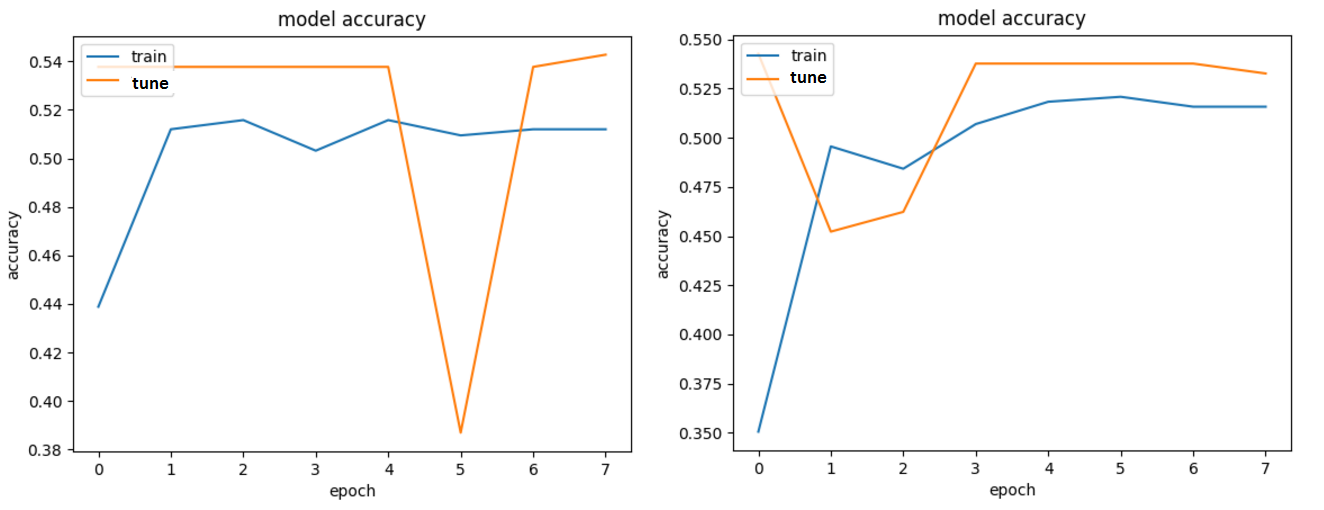
\includegraphics[width=\columnwidth]{graph}}
\caption{Accuracy for training and tuning sets on test 4 (left) and test 5 (right).}
  \label{accuracy}
  \end{center}
  \vskip -0.2in
\end{figure}


\begin{figure}[ht]
  \vskip 0.2in
  \begin{center}
\centerline{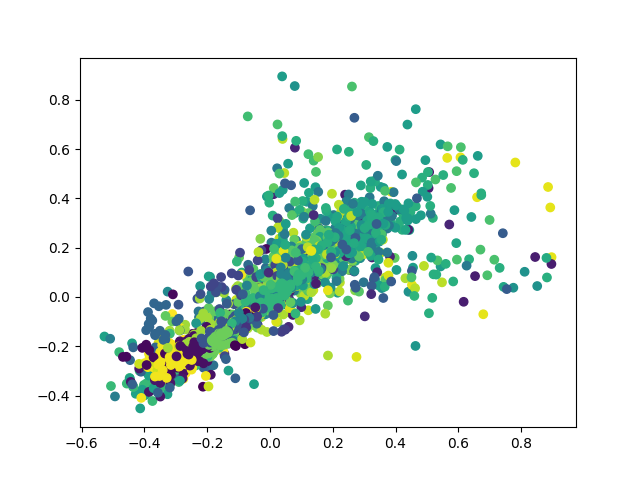
\includegraphics[width=\columnwidth]{plot2}}
\caption{Cluster assignment of patches for img7 (type 1) using the codebook.}
  \label{cluster}
  \end{center}
  \vskip -0.2in
\end{figure}

\begin{figure}[ht]
  \vskip 0.2in
  \begin{center}
  \centerline{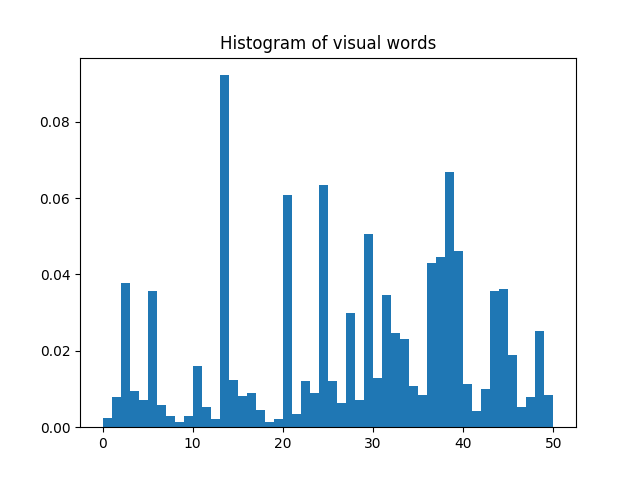
\includegraphics[width=\columnwidth]{hist2}}
  \caption {Histogram of patches for img7 (type 1) using the codebook.}
  \label{histogram}
  \end{center}
  \vskip -0.2in
\end{figure}



\section{Discussion}
Tests 1 through 3 (Table 2.) had the same architecture implementation except for variation in the number of kernels for the convolutional layer and the output size of the FC layer. All three tests resulted in the same score on the tuning set, which was higher than the score on training set in all cases. This indicates that increasing the  number of layers or output size of FC did not increase the performance of our model.

With the same number of kernels for convolutional layer and output size of FC layer, with a Dropout Layer added to the architecture, test 4 gave the same max accuracy as test 3, however scores better on the tune set, and in fact this is the best score we got across all the tests on the tuning set. 



 
From test 4 to test 5, we increased the complexity of our model with
architeture CNN2 (Table 1.)  by adding another Convolutional Layer
with K=16. This led to a decrease in the tuning score, the resulting
accuracy rate scored on the training and tuning sets in tests 4 and 5
is shown by fig. (8). With the same architecture of 2 Convolutional layers, comparing test 5 and test 6 shows that with fewer layers, our model performed worse on the tuning set and seemed to overfit the dataset with a higher score on the training set. Similarly, with another Convolutional layer added in CNN3, comparing test 7 with 5 shows worse performance on the tuning set and overfitting with higher train score. However, test 8 indicates that an increase in the number of kernels in the first Convolutional layer gave better accuracy rate on the tuning set. From our results in Table (2) and the graphs in Figure (10), we can see that applying the model to the tuning set often outperforms the training set, so we conducted test 10 and 11 with a smaller number of epochs (5) and increased the batch size in test 10 (32). However, results show equivalent accuracy rates on both train and tuning sets. 


\begin{table}[h!]
 \caption{Results on the training and test sets for CNN, BOWs and MLP}
 \label{tab:format-se}
 \vskip 0.15in
 \begin{center}
 \begin{small}
 \begin{sc}
 \begin{tabular}{lccr}
 \hline
 \abovespace\belowspace
Method & Train Score & Tune Score & Time\\
\hline
\abovespace\belowspace
CNN & 0.5183 & 0.5440 & 9.6548\\
\hline
\abovespace\belowspace
BOWs & 0.5813 & 0.5678 & 2.8761\\
\hline
\abovespace\belowspace
MLP & 0.9130 & 0.4438 & 1.4576\\
\hline
 \end{tabular}
 \end{sc}
 \end{small}
 \end{center}
 \vskip -0.1in
\end{table}

Choosing the best performance seen in test 4, we conducted test 12: an
architecture set up exactly the same as in test 4 except without the
BatchNormalization layer. Even though the scores on the training set
are the same, with BatchNormalization test 4 performed better on the
tuning set. Observing the kernel weights of the convolutional layer in
Fig. (4), we conducted an additional test 13 with CNN1 architecture but increased receptive field size F = 5 to see if a bigger kernel can extract more useful features of the images. This resulted in a similar score on the training set but a lower score on the tuning set (.5377 versus .5427). 


We implemented CNN1 with batch size=10, epoch=8 on the test set and yielded an accuracy rate=.5440, close to our score on the tuning set (.5427) in 39.8926s fitting time. Comparing with other 2 methods, BOWs gained a better accuracy rate (.5678) on the test set, while MLP gave a lower score of (.4438). Both BOWs and MLP produced a better score on the training set, especially MLP (training accuracy = .9130), suggesting that the classifiers overfitted. In comparison with the average accuracy rate on the test set among all three classifiers (.5185) our CNN gives a score better than average (even though the score is only 64.26\% better than chance (.3333). Fitting time-wise, the method BOWs gives a better performance with better score than CNN (39.8926 versus 2.8761), however the process of computing the histogram from the codebook took a lot of waiting time. 

Through tweaking with the choice of number of layers, size of layers and
choice of hyperparameters, we observed in our experiments that the increase in number of
layers, especially convolutional layer, and increase in number of
layer's output size increased the fitting time. 

\section{Conclusion}
By conducting multiple tests varying the architecture of the model and the hyperparameters for the CNN, we found that the model performed best on the tuning set with CNN1. Even though the rate obtained on the testing set (.5440) is only 63.21\% better than chance, comparing with other methods we tried, CNN performed better than average (.5185). The best performance across CNN, BOWs and MLP is BOWs with a codebook constructed by segmenting 5x5 patches from each image and using k-means to determine 50 cluster centers (accuracy rate = .5678). However, this method demands a lot of time for computing the histograms for each image to build the training set.

While further engineering the CNN by adjusting the number of layers, layer output sizes and other hyperparameters can help increase the accuracy rate, data augmentation is also important.  The image processing algorithm could work better by eliminating similar images in our dataset.  Another step is to refine the initial ROI such that it matches the cervix boundary more closely.  This could be done by using prior shape information, combining feature values measured along the shape boundary such as edges. While our current segmentation algorithm zeroed out the regions affected by strong reflectors already, a better next step would be to propagate surrounding pixels into specular regions, creating smooth filling of the image \cite{autodetect}.

Further work to boost the performance of the classifier is trying out
the fine-tuning approach. Knowing that a pre-trained CNN model have
already learned features relevant to our classification problem such
as edges, regional features, we can improve our model by taking
advantage of the pre-trained model’s resulting weights An
implementation of this would be instantiating the convolutional base
with the weights of a pre-trained CNN such as VGG16 \cite{vgg16}, freezing all the layer of VGG16 up to the last convolutional block, then add our previously defined FC model on top (\href{https://blog.keras.io/building-powerful-image-classification-models-using-very-little-data.html}{keras blog}).   


\bibliographystyle{icml2014}
\bibliography{dginzbu1-lngoquy1}


\end{document}